\documentclass[11pt]{beamer}

\usepackage[utf8]{inputenc}
\usepackage{tikz}
\usepackage{graphicx}
\usepackage{amsmath}
\usepackage{color}
\usepackage{xcolor}

\usetikzlibrary{calc, positioning, arrows}

\logo{
\includegraphics[scale=.5]{TUM_Logo.eps}}
\title[Short version]{Unidirectional NCM}
\subtitle[short version]{Implementation}
\date[2021]{Network Coding}
\author[Andreas Bauer, Lion Steger]{Andreas Bauer, Lion Steger}
\institute[Technische Universität München]{Technische Universität München}

\begin{document}
	\frame{\maketitle}
	
	\begin{frame}{Initial State}
		\begin{itemize}
			\item two neighbors communicating form a session
			\item sessions are always bidirectional (have two flows in opposite directions)
			\item multiple packets are called a generation
			\item sessions manage multiple generations inside a generation window
			\item sender and receiver hold state $ \begin{bmatrix}
				C \\ B
			\end{bmatrix} = \begin{bmatrix}
				1 C \\ A C
			\end{bmatrix} $ per generation where $ C $ is the coding matrix
			\item coding matrix are split for the two directions, $A$ accordingly
			\[
			\left[
			\begin{array}{c|c}
			C_s & 0 \\ \hline
			0 & C_r \\
			\end{array}
			\right]
			\]
			\item this might be overly complicated?
		\end{itemize}
	\end{frame}

	\begin{frame}{Our State}
		\begin{itemize}
			\item two neighbors communicating form two sessions
			\item one session for each unidirectional information flow
			\item coding matrix is used for only one direction by setting the dimension of one side to zero
			\[
			\left[
			\begin{array}{c|c}
			C &  \\ \hline
			  &  \\
			\end{array}
			\right]
			\]
		\end{itemize}
	\end{frame}

	\begin{frame}{Timeline}
		\begin{itemize}
			\item understand the code
			\item begin implementing our own, unidirectional versions of \texttt{generation.c} and \texttt{session.c}
			\item write unit tests that run the code on one device locally instead of real communication over radio
			\item leverage various tools such as CI, code coverage tests and memory checks
			\item integrating the new session/generation functionality into the existing code and conduct real-world tests
		\end{itemize}
	\end{frame}

	\begin{frame}{Our (Non-)Changes}
		Implementing this seems simple\ldots right?
		\begin{itemize}
			\item using the full coding matrix without changes to librlnc!
			\item no changes to the neighbor/link quality functionality or main event loop files
			\item rewrite only the calls to the session and generation API:
			\begin{itemize}
				\item acknowledgment and re-transmission scheme
				\item generation window advancement
				\item packet statistics
				\item header structures
				\item utility functions (e.g.\ remaining space)
				\item meta structures used to avoid dependencies to ncm code
			\end{itemize}
		\end{itemize}
	\end{frame}

	\begin{frame}{Acknowledgment Scheme}
		Fundamental principles:
		\begin{itemize}
			\item coded packets are sent for every generation until they are acknowledged
			\item each received coded packet triggers an acknowledgment
			\item acknowledgments contain the dimensions of all generations in the current window
			% using this state info, sender node can determin if it still needs to transmit coded packets
		\end{itemize}
	\end{frame}

	\begin{frame}{Generation Advancement Scheme}
		A generation is considered complete if:
		\begin{itemize}
			\item \ldots all packets are sent and acknowledged (Source)
			\item \ldots all packets are received and decoded (Destination)
		\end{itemize}
	\end{frame}

	\begin{frame}{Generation Advancement Scheme}
		\begin{figure}
			\centering
			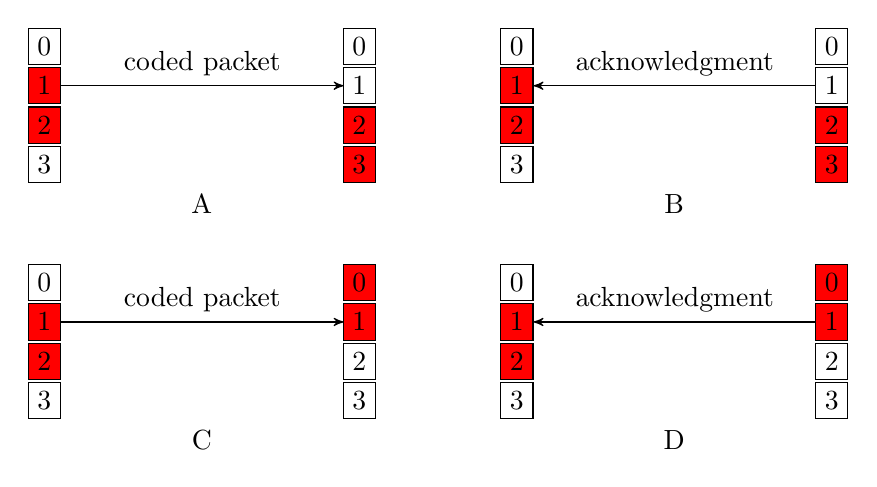
\begin{tikzpicture}[>=stealth',t/.style={minimum width=1cm, minimum height=0.7cm}]
				\node[draw] at (0,0) {3};
				\node[draw,fill=red] at (0,0.5) {2};
				\node[draw,fill=red] (s) at (0,1) {1};
				\node[draw] at (0,1.5) {0};
				\node[draw] at (4,0) {3};
				\node[draw] at (4,0.5) {2};
				\node[draw,fill=red] at (4,1) {1};
				\node[draw,fill=red] at (4,1.5) {0};
				\coordinate (r) at (3.8,1);
				\draw[->] (s) -- node[above] {coded packet} (s-|r);
				\node[] at (2,2.5)  {A};
				
				\node[draw] at (0,3) {3};
				\node[draw,fill=red] at (0,3.5) {2};
				\node[draw,fill=red] (s) at (0,4) {1};
				\node[draw] at (0,4.5) {0};
				\node[draw,fill=red] at (4,3) {3};
				\node[draw,fill=red] at (4,3.5) {2};
				\node[draw] at (4,4) {1};
				\node[draw] at (4,4.5) {0};
				\coordinate (r) at (3.8,1);
				\draw[->] (s) -- node[above] {coded packet} (s-|r);
				\node[] at (2,-0.5)  {C};
				
				\node[draw] at (6,0) {3};
				\node[draw,fill=red] at (6,0.5) {2};
				\node[draw,fill=red] (s) at (6,1) {1};
				\node[draw] at (6,1.5) {0};
				\node[draw] at (10,0) {3};
				\node[draw] at (10,0.5) {2};
				\node[draw,fill=red] at (10,1) {1};
				\node[draw,fill=red] at (10,1.5) {0};
				\coordinate (r) at (9.8,1);
				\draw[<-] (s) -- node[above] {acknowledgment} (s-|r);
				\node[] at (8,2.5)  {B};
				
				\node[draw] at (6,3) {3};
				\node[draw,fill=red] at (6,3.5) {2};
				\node[draw,fill=red] (s) at (6,4) {1};
				\node[draw] at (6,4.5) {0};
				\node[draw,fill=red] at (10,3) {3};
				\node[draw,fill=red] at (10,3.5) {2};
				\node[draw] at (10,4) {1};
				\node[draw] at (10,4.5) {0};
				\coordinate (r) at (9.8,1);
				\draw[<-] (s) -- node[above] {acknowledgment} (s-|r);
				\node[] at (8,-0.5)  {D};
			\end{tikzpicture}\label{fig:figure}
		\end{figure}
	\end{frame}

	\begin{frame}{Testing}
		We designed several tests for:
		\begin{itemize}
			\item initializing sessions and generations
			\item correct behavior of generation sequence numbers in edge cases
			\item logging of session statistics
			\item basic encoding, sending, receiving and decoding of frames
			\item multiple random packets sent in a loop
		\end{itemize}
	\end{frame}
\end{document}